\documentclass[marklength=0mm,
    coverwidth=210mm,
    coverheight=297mm,
    bleedwidth=3mm,
    spinewidth=5.9mm,cmyk]{bookcover}

\usepackage{blindtext}
\usepackage[T1]{fontenc}
\usepackage[default]{opensans}
\usepackage{graphicx}
\usepackage{pbox}
\usepackage{setspace}
\usepackage[misc]{ifsym}
\usepackage{microtype}
\usepackage{tikz,ifthen}
\usepackage{xcolor}
\usepackage{pgfplots}
\usepackage{colortbl}
%\usepackage{pifont}

\definecolor{frontcolor}{cmyk}{1,0.65,0,0}
\definecolor{frontcolor2}{cmyk}{0.8,0.52,0,0}
\definecolor{spinecolor}{cmyk}{0,0.8,0.9,0}

\begin{document}

%back cover
\setbookcover{bgcolor}{back}{%
color=white,
}

\setbookcover{fgsecond}{back}{%
\vspace{2.5cm}
\centering
\vfill
}

\setbookcover{fgfirst}{back}{%
\centering
\begin{minipage}[c]{.8\textwidth}
{
\vspace*{3cm}

\begin{minipage}{1\linewidth}

{ \rule{\linewidth}{1pt}}
\vspace{5mm}
%\begin{center}
%\textbf{Abstract}\\
%\end{center}
\begin{abstract}
Multinational enterprises may use income shifting techniques such as strategic transfer pricing and debt shifting to reduce their global tax burden. Due to a comparably low corporate taxation, Switzerland is a seemingly suitable location for tax planning strategies. The thesis at hand examines income shifting among multinational enterprises headquartered in Switzerland in a quantitative manner and provides indirect evidence of income shifting. Using a large panel dataset of foreign subsidiaries of Swiss parent firms and employing a fixed-effects regression approach, the estimated semi-elasticity of pre-tax income with respect to the statutory tax rate differential between the parent firm and the subsidiary in the benchmark specification is -1.458. This estimate is highly significant and larger than the estimates in comparable papers using European samples. Additionally, this thesis shows that income shifting activities between the parent firm and the subsidiary increase with the parent's ownership share in the subsidiary and the firm size of the subsidiary. Hence, Swiss multinational enterprises preferably shift income using large, wholly-owned subsidiaries.
\end{abstract}
\end{minipage}
}
\vspace*{8.7cm}

%---MIDDLE---
\begin{minipage}{0.5\linewidth}
{\Letter}\\
Rafael Daniel Schlatter\\
Weidstrasse 50\\
4416 Bubendorf\\
Switzerland\\
           
11-707-668\\
Business Administration\\
rafaelschlatter@gmail.com\\

\textit{Supervisor}:
Benedikt Bisig\\
\textit{Expert}: Prof. Dr. Dieter Pfaff\\

Oslo, Jul 17, 2017
\end{minipage}
%
\begin{minipage}{0.5\linewidth}
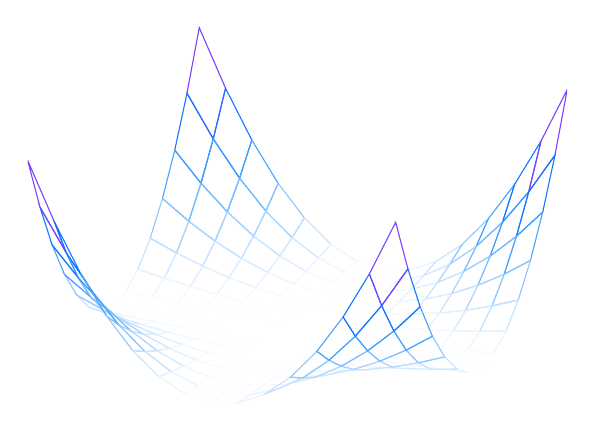
\begin{tikzpicture}[scale=1]
	\begin{axis}[
		axis lines=none,
		samples=15, domain=-4:4,
		xtick=data, ytick=data,
		colormap/cool,
	]
		\addplot3[mesh] {x^2*y^2};
	\end{axis}
\end{tikzpicture}
\end{minipage}

\vspace{2cm}

%---BOTTOM---
\begin{minipage}{0.6\linewidth}
\includegraphics[height=17mm]{uzh_logo_e_pos.pdf}
\end{minipage} \hspace{15pt}
%
\begin{minipage}{0.02\linewidth}
    \rule{1pt}{30pt}
\end{minipage} \hspace{-5pt}
%
\begin{minipage}{0.4\linewidth}
\vspace{5pt}
\small{Department of Business Administration\\ \textit{Chair for Managerial Accounting}}
\end{minipage}
\end{minipage}
}

%front cover
\setbookcover{bgcolor}{front}{%
color=black,
}

\setbookcover{fgsecond}{front}{%
\vspace{0cm}
\centering

\vfill
}

\setbookcover{fgfirst}{front}{%
\centering
\begin{minipage}[c]{.8\textwidth}

\vspace*{3cm}

{\color{white} \rule{\linewidth}{1mm}}
\vspace{5mm}

\textcolor{white}{\fontsize{24.5pt}{15pt}\selectfont The impact of tax differentials on pre-tax income of Swiss multinational enterprises}

\vspace{5mm}
{\color{white} \rule{\linewidth}{1pt}}
\vspace{5mm}

\large{\textcolor{white}{Master Thesis \hfill Oslo\\ Rafael Daniel Schlatter \hfill Jul 17, 2017}} 
\vspace{5mm}


\vspace{7cm}


\begin{tikzpicture}[scale=0.4]
	\begin{axis}[
		axis lines=none,
		samples=5, domain=-4:4,
		xtick=data, ytick=data,
		colormap/hot,
	]
		\addplot3[surf] {x*y};
	\end{axis}
\end{tikzpicture}
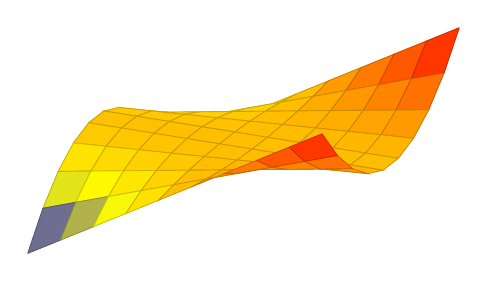
\begin{tikzpicture}[scale=0.8]
	\begin{axis}[
		axis lines=none,
		samples=10, domain=-4:4,
		xtick=data, ytick=data,
		colormap/hot,
	]
		\addplot3[surf] {x*y^2};
	\end{axis}
\end{tikzpicture}
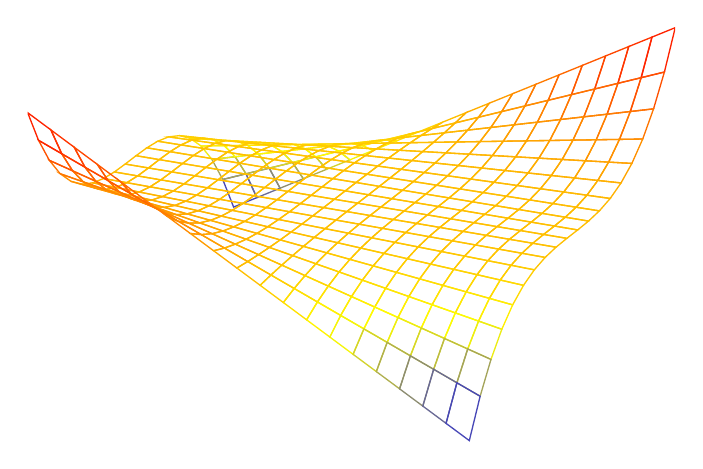
\begin{tikzpicture}[scale=1.2]
	\begin{axis}[
		axis lines=none,
		samples=20, domain=-200:200,
		xtick=data, ytick=data,
		colormap/hot,
	]
		\addplot3[mesh] {x*y^3};
	\end{axis}
\end{tikzpicture}

\vspace{3cm}

%---BOTTOM---
\begin{minipage}{0.6\linewidth}
\includegraphics[height=17mm]{uzh_logo_e_neg.eps}
\end{minipage} \hspace{15pt}
%
\begin{minipage}{0.02\linewidth}
    \color{white}{\rule{1pt}{30pt}}
\end{minipage} \hspace{-5pt}
%
\begin{minipage}{0.4\linewidth}
\vspace{5pt}
\small{\textcolor{white}{Department of Business Administration}\\ \textit{\textcolor{white}{Chair for Managerial Accounting}}}
\end{minipage}
\end{minipage}
}

%spine
\setbookcover{bgcolor}{spine}{%
color=spinecolor,
}

\setbookcover{fgfirst}{spine}{
\vfill
\centering
\small
\rotatebox[origin=c]{270}{\textcolor{white}{%\fontfamily{ppl}\selectfont 
The impact of tax differentials on pre-tax income of Swiss multinational enterprises} \hspace{4cm}

\begin{tabular}{!{\color{white}\vrule}c !{\color{white}\vrule} c !{\color{black}\vrule} c !{\color{black}\vrule}}
\textcolor{white}{Master Thesis}&\textcolor{white}{R. D. Schlatter} &University of Zurich
\end{tabular}}
\vfill}

\makebookcover
\end{document}
